\let\negmedspace\undefined
\let\negthickspace\undefined
\documentclass[journal]{IEEEtran}
\usepackage[a5paper, margin=10mm, onecolumn]{geometry}
%\usepackage{lmodern} % Ensure lmodern is loaded for pdflatex

\setlength{\headheight}{1cm} % Set the height of the header box
\setlength{\headsep}{0mm}     % Set the distance between the header box and the top of the text

\usepackage{gvv-book}
\usepackage{gvv}
\usepackage{cite}
\usepackage{amsmath,amssymb,amsfonts,amsthm}
\usepackage{algorithmic}
\usepackage{graphicx}
\usepackage{textcomp}
\usepackage{xcolor}
\usepackage{txfonts}
\usepackage{listings}
\usepackage{enumitem}
\usepackage{mathtools}
\usepackage{gensymb}
\usepackage{comment}
\usepackage[breaklinks=true]{hyperref}
\usepackage{tkz-euclide} 
\usepackage{listings}
% \usepackage{gvv}                                        
\def\inputGnumericTable{}                                 
\usepackage[latin1]{inputenc}                                
\usepackage{color}                                            
\usepackage{array}                                            
\usepackage{longtable}                                       
\usepackage{calc}                                             
\usepackage{multirow}                                         
\usepackage{hhline}                                           
\usepackage{ifthen}                                           
\usepackage{lscape}
\begin{document}

\bibliographystyle{IEEEtran}
\vspace{3cm}

\title{1.6.12}
\author{EE24BTECH11033 - Kolluru Suraj}
% \maketitle
% \newpage
% \bigskip
{\let\newpage\relax\maketitle}
\renewcommand{\thefigure}{\theenumi}
\renewcommand{\thetable}{\theenumi}
\setlength{\intextsep}{10pt} % Space between text and floats
\numberwithin{equation}{enumi}
\numberwithin{figure}{enumi}
\renewcommand{\thetable}{\theenumi}
\textbf{Question:}\\
Point $ \myvec{-4, 2}$ lies on the line segment joining the points $\vec{A}\myvec{-4\\ 6}$  and  $\vec{B}\myvec{-4\\ -6}$.
\\
\solution\\
\begin{table}[h!]
  \centering
  \begin{tabular}{ |c| c|}
    \hline
    \textbf{point}  &  \textbf{Coordinates}\\
    \hline
    $\vec{A}$ & $\brak{-4,6}$ \\
    \hline
    $\vec{B}$ & $\brak{-4,-6}$\\
    \hline
    $\vec{C}$ & $\brak{-4,2}$\\
    \hline
\end{tabular}    


  \caption{variables used}
  \label{tabQuestion-1.6.12}
\end{table}


Points $\vec{A}, \vec{B}, \vec{C}$ are defined to be collinear if 
		\begin{align}
			\label{eq:line-rank-2}
			\rank{\myvec{\vec{B}-\vec{A}& \vec{C}-\vec{A}}} = 1
		\end{align}

  \begin{align}
 \vec{B}-\vec{A}=\myvec{ 0\\ -12}
\end{align}
\begin{align}
 \vec{C}-\vec{A}=\myvec{ 0\\ -4}
\end{align}\\
The collinearity matrix can be expressed as
 \begin{align}
			    \myvec{0 & 0\\-12 & -4 }  
\end{align}
which is a rank 1 matrix.
To find the ratio which $\vec{C}$ divides $\vec{A},\vec{B}$. Using section formula,
\begin{align}
         \myvec{-4\\2} &=\frac{{\myvec{-4\\6}+k\myvec{-4\\-6}}}{1+k}\\
	 \implies 2k\myvec{0 \\ 4} &=\myvec{0 \\ 4}
	 \\
	 \text{or, } k &= \frac{1}{2}.
\end{align}

\begin{figure}[h!]
   \centering
   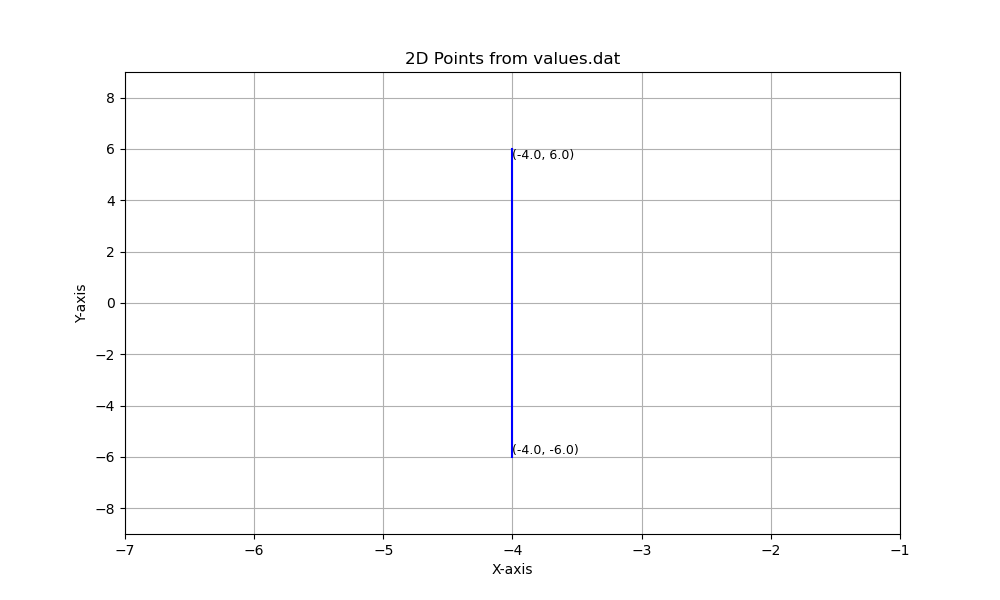
\includegraphics[width=0.7\linewidth]{figs/Figure_1.png}
   \caption{Line connecting $AB$}
   \label{stemplot}
\end{figure}
	


\end{document}

